\begin{table}[t]
    \centering
    \begin{tabular}{cccc}
    \hspace{-5mm}
         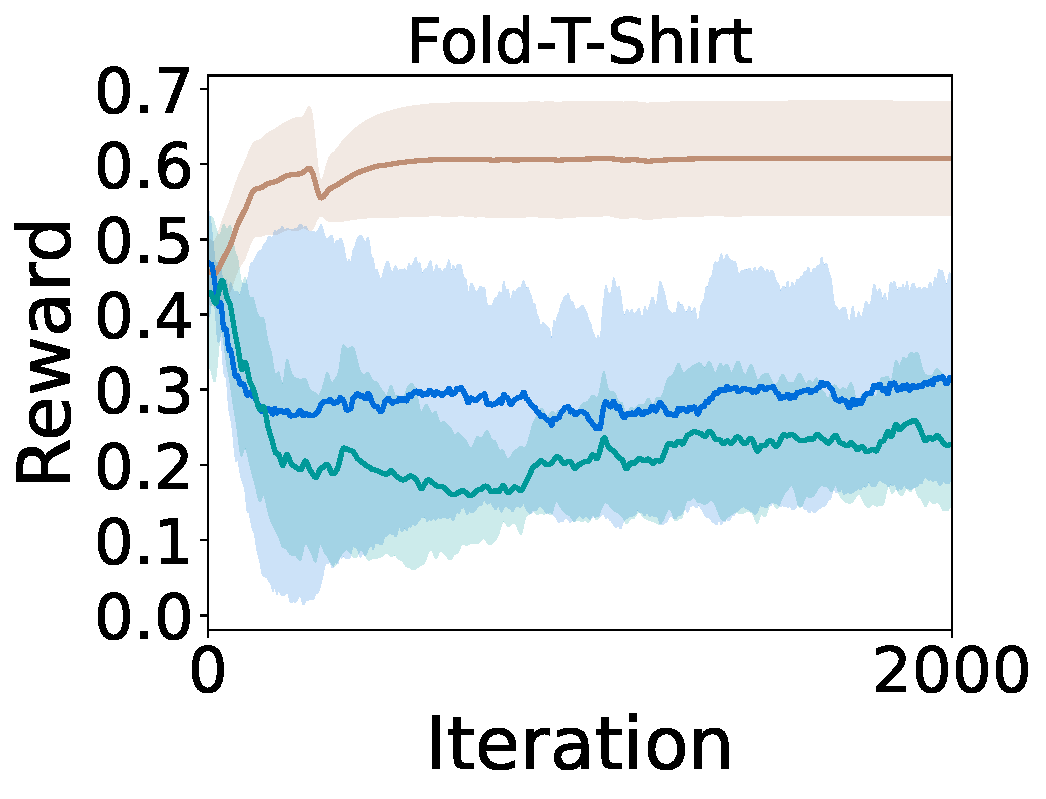
\includegraphics[width=0.23\textwidth]{iclr2023/figs/rl_training_curve/fold_tshirt.pdf}
         &
        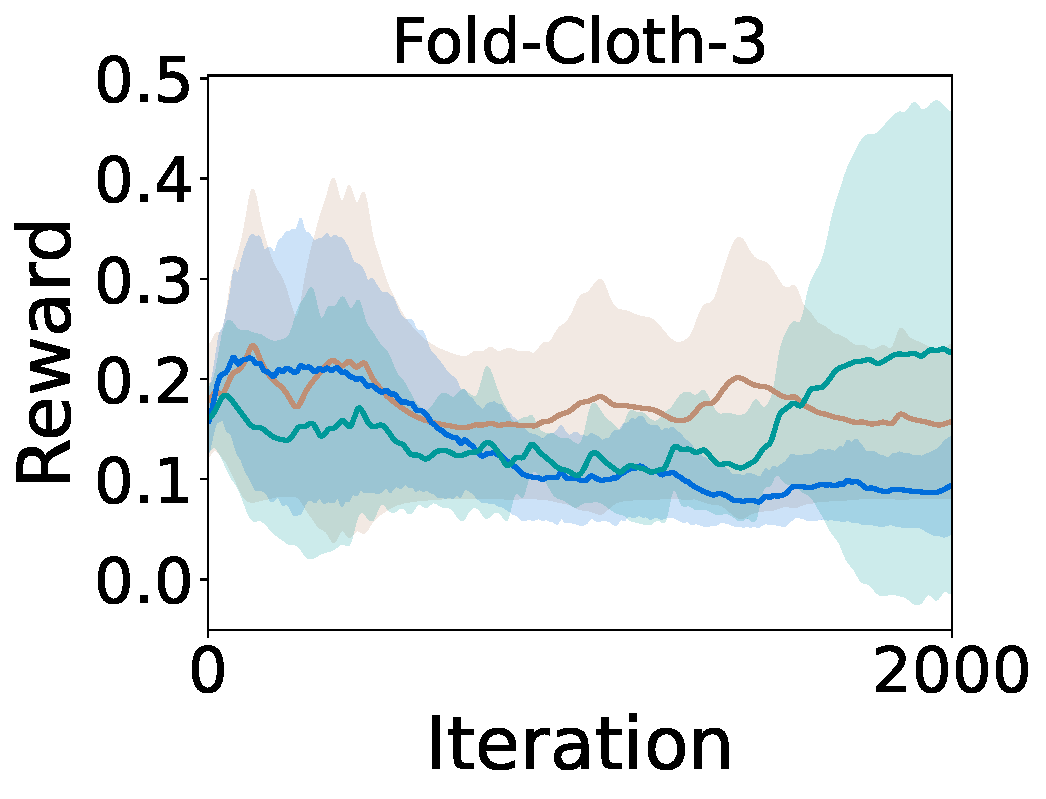
\includegraphics[width=0.23\textwidth]{iclr2023/figs/rl_training_curve/fold_cloth3.pdf}
         &
        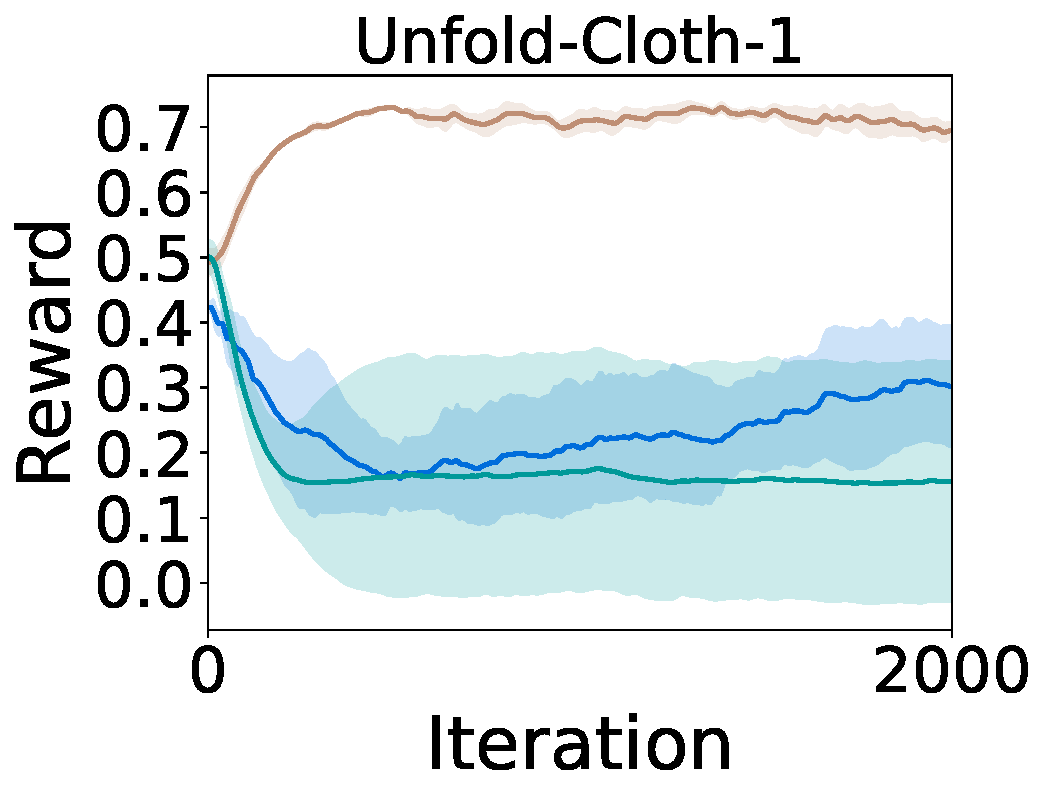
\includegraphics[width=0.23\textwidth]{iclr2023/figs/rl_training_curve/unfold_cloth1.pdf}
         &
        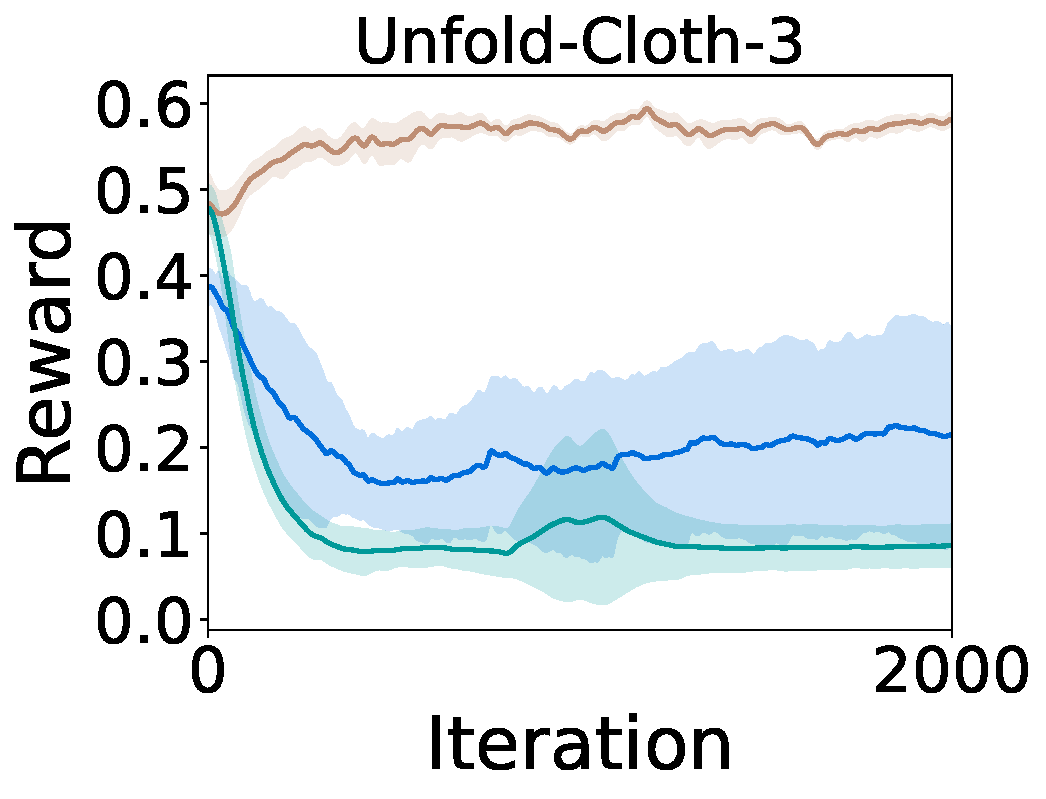
\includegraphics[width=0.23\textwidth]{iclr2023/figs/rl_training_curve/unfold_cloth3.pdf}
         \\
             \hspace{-5mm}
        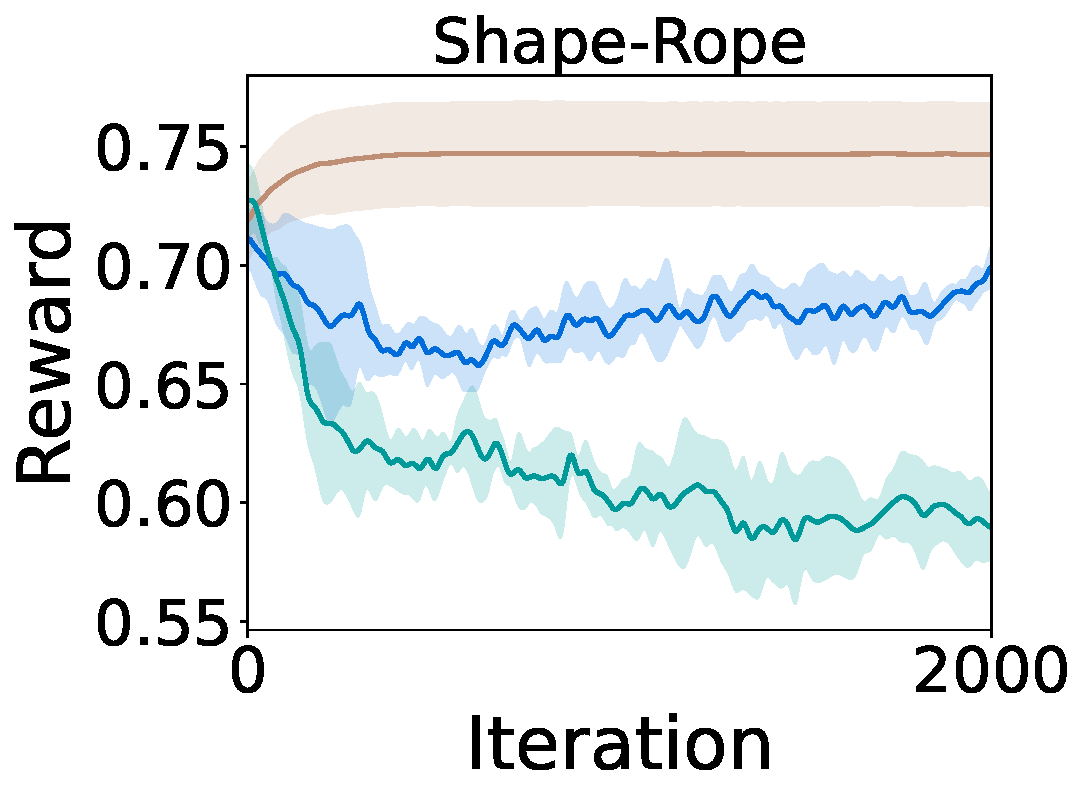
\includegraphics[width=0.23\textwidth]{iclr2023/figs/rl_training_curve/shape_rope.pdf}
         &
        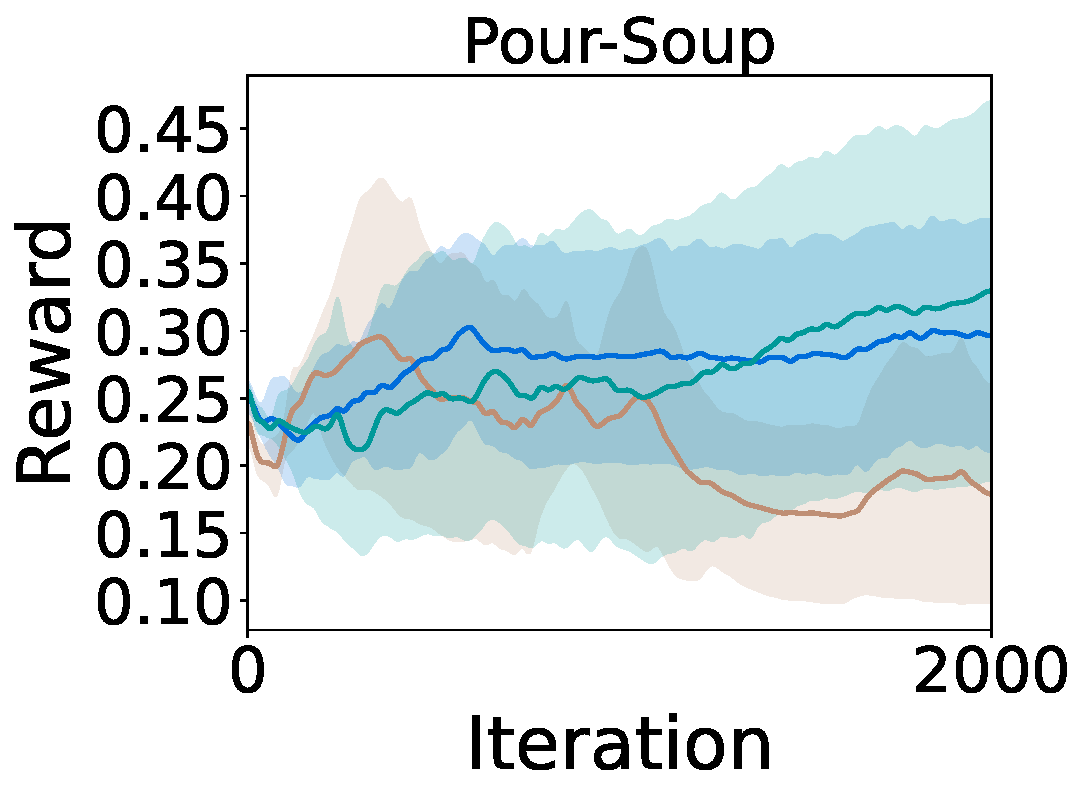
\includegraphics[width=0.23\textwidth]{iclr2023/figs/rl_training_curve/pour_soup.pdf}
         &
        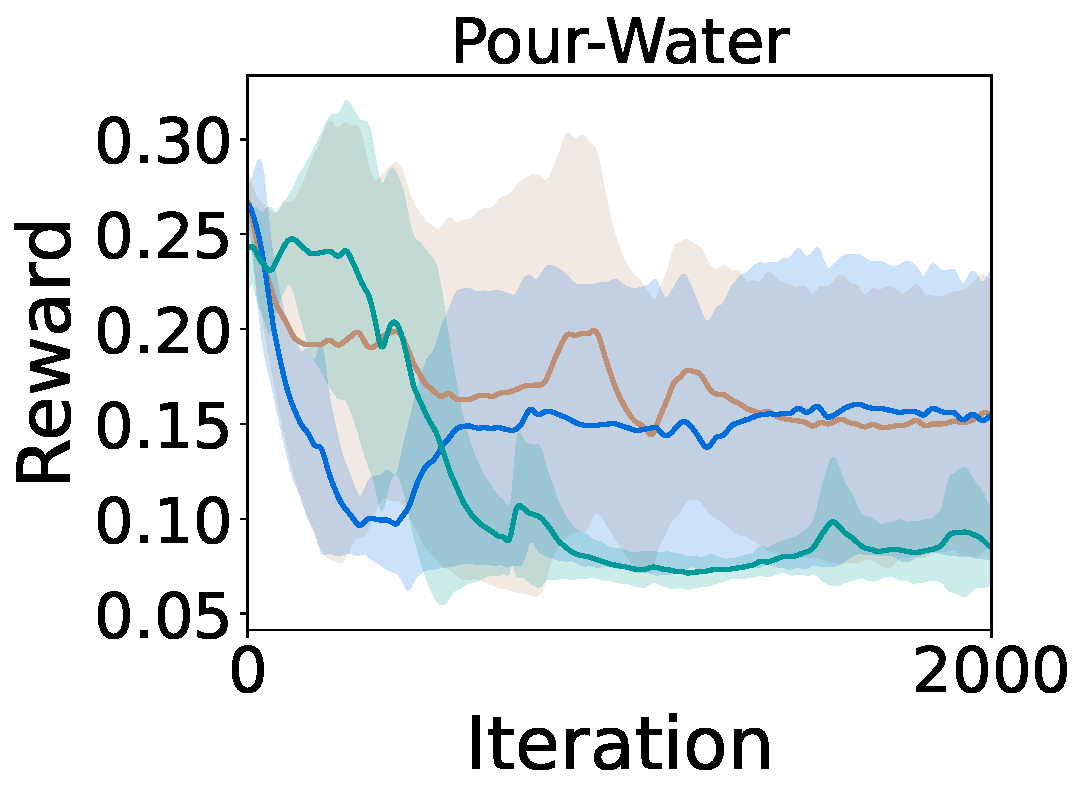
\includegraphics[width=0.23\textwidth]{iclr2023/figs/rl_training_curve/pour_water.pdf}
         &       
         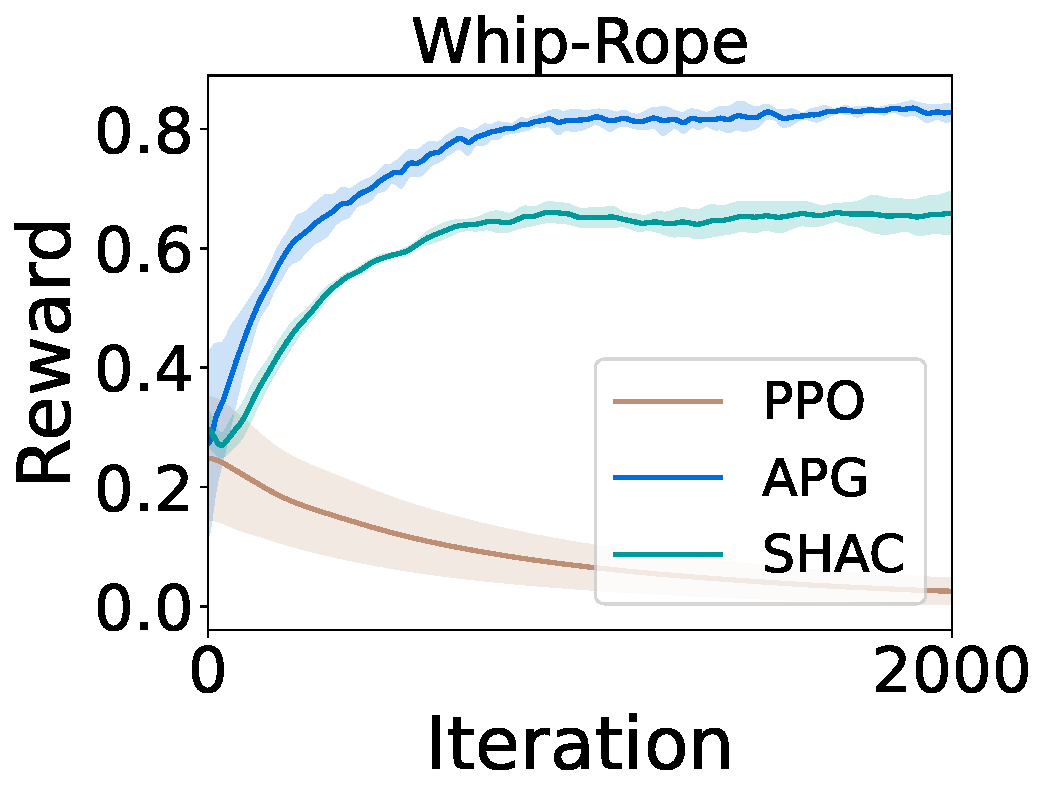
\includegraphics[width=0.23\textwidth]{iclr2023/figs/rl_training_curve/whip_rope.pdf}

    \end{tabular}
    \captionof{figure}{\textbf{Learning curves of three benchmarked RL algorithms: PPO, APG, and SHAC.} The y-axis shows the episode reward, scaled from 0 to 1, with larger values being closer to the goal state. The x-axis is the number of training iterations. All methods are trained in the same number of batched environments. We report the mean and variance of the performance for 5 seeds and each seed has 20 rollouts with different initializations. We refer the readers to Table \ref{table:RL_results} for the numerical results in the appendix.
    }
    \label{tab:rl_learning_curves}
\end{table}